\chapter{Estado de Arte}
\label{sec:estado-arte}

Neste capítulo será feita uma análise de algumas plataformas existentes para recolha de dados em estratégias de inbound marketing. A recolha de informação nos dias de hoje tem um grande impacto na forma como os negócios são feitos, principalmente na internet. Neste contexto, serão analisadas algumas das soluções que partilham funcionalidades semelhantes com o que vai ser desenvolvido.\\
Como referido no capítulo anterior, o modelo de negócio da plataforma é \gls{b2b} e neste sentido as caracteristicas analisadas serão focadas na segmentação de dados, integração com serviços externos, planos de pagamento e funcionalidades do \textit{back office}.
Seguindo uma das estratégias de inbound marketing, o método de envio de formações e recolha de dados será através da formulários online e por isso mesmo algumas características associadas à experiencia do utilizador, como por exemplo a personalização do formulário, serão também analisadas.


As plataformas a analisar serão o SurveyMonkey\cite{surveymonkey}

Após a apresentação destas ferramentas será feita uma análise das vantagens e desvantagens de cada uma, assim como a comparação de funcionalidades.


\section{SurveyMonkey}
\label{surveyMonkey}

O SurveyMonkey é um \acrfull{saas} de criação de questionários online. É necessário criar conta para aceder às funcionalidades da plataforma, dando a opção de utilizar serviços externos para esse efeito (e. g. Facebook\cite{face}, LinkedIn\cite{linkedin}), como podemos ver na Figura \ref{fig:surveymonkey-singin}. O SurveyMonkey é uma plataforma que dispões de diversos planos de pagamento, e por isso mesmo, apesar de estar disponível um plano gratuito, tem acesso apenas a algumas das funcionalidades e em cada questionário, no máximo, poderá ter 10 perguntas ou elementos. 

\begin{figure}[ht!]
	\begin{center}
		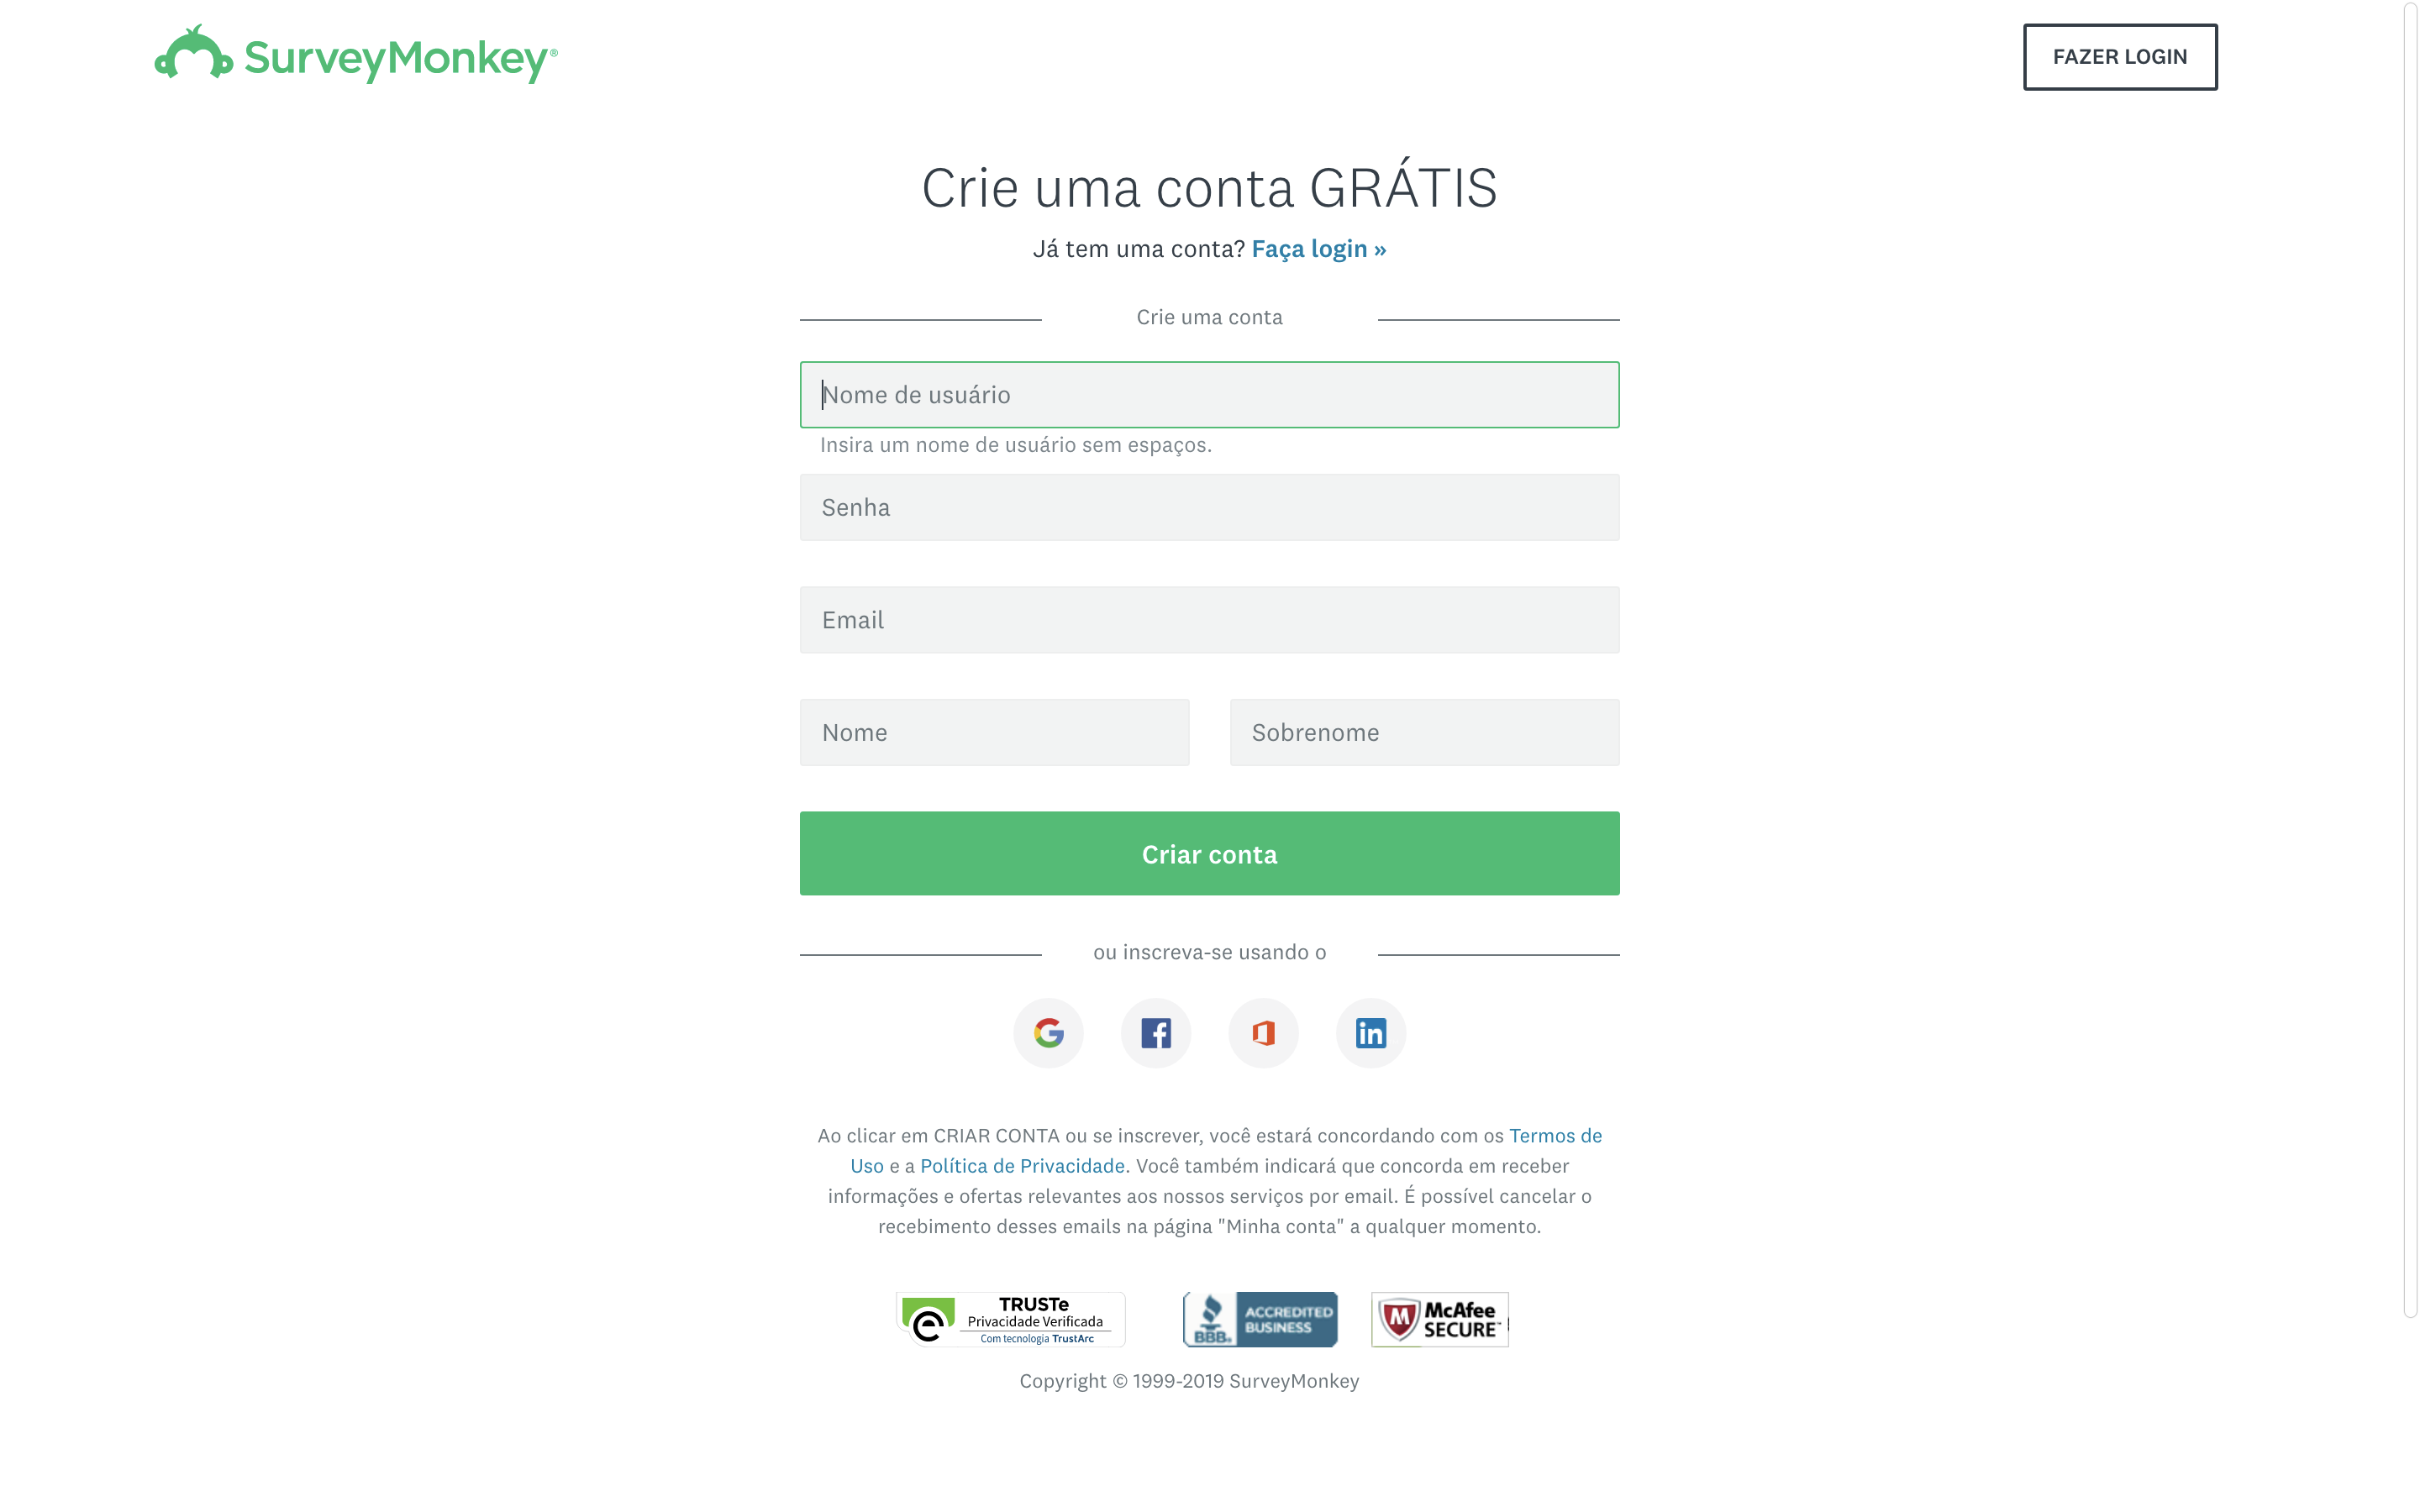
\includegraphics[width=1\textwidth]{img/surveymonkey-singin}
		\caption{SurveyMonkey - Registro }
		\label{fig:surveymonkey-singin}
	\end{center}
\end{figure}

\newpage

No painel principal, como podemos ver na Figura \ref{fig:survey-dashboard} temos acesso rápido aos questionários recentes e a algumas métricas sobre os mesmos. Outra forma será aceder aos questionários do utilizador através da barra de navegação. 


\begin{figure}[ht!]
	\begin{center}
		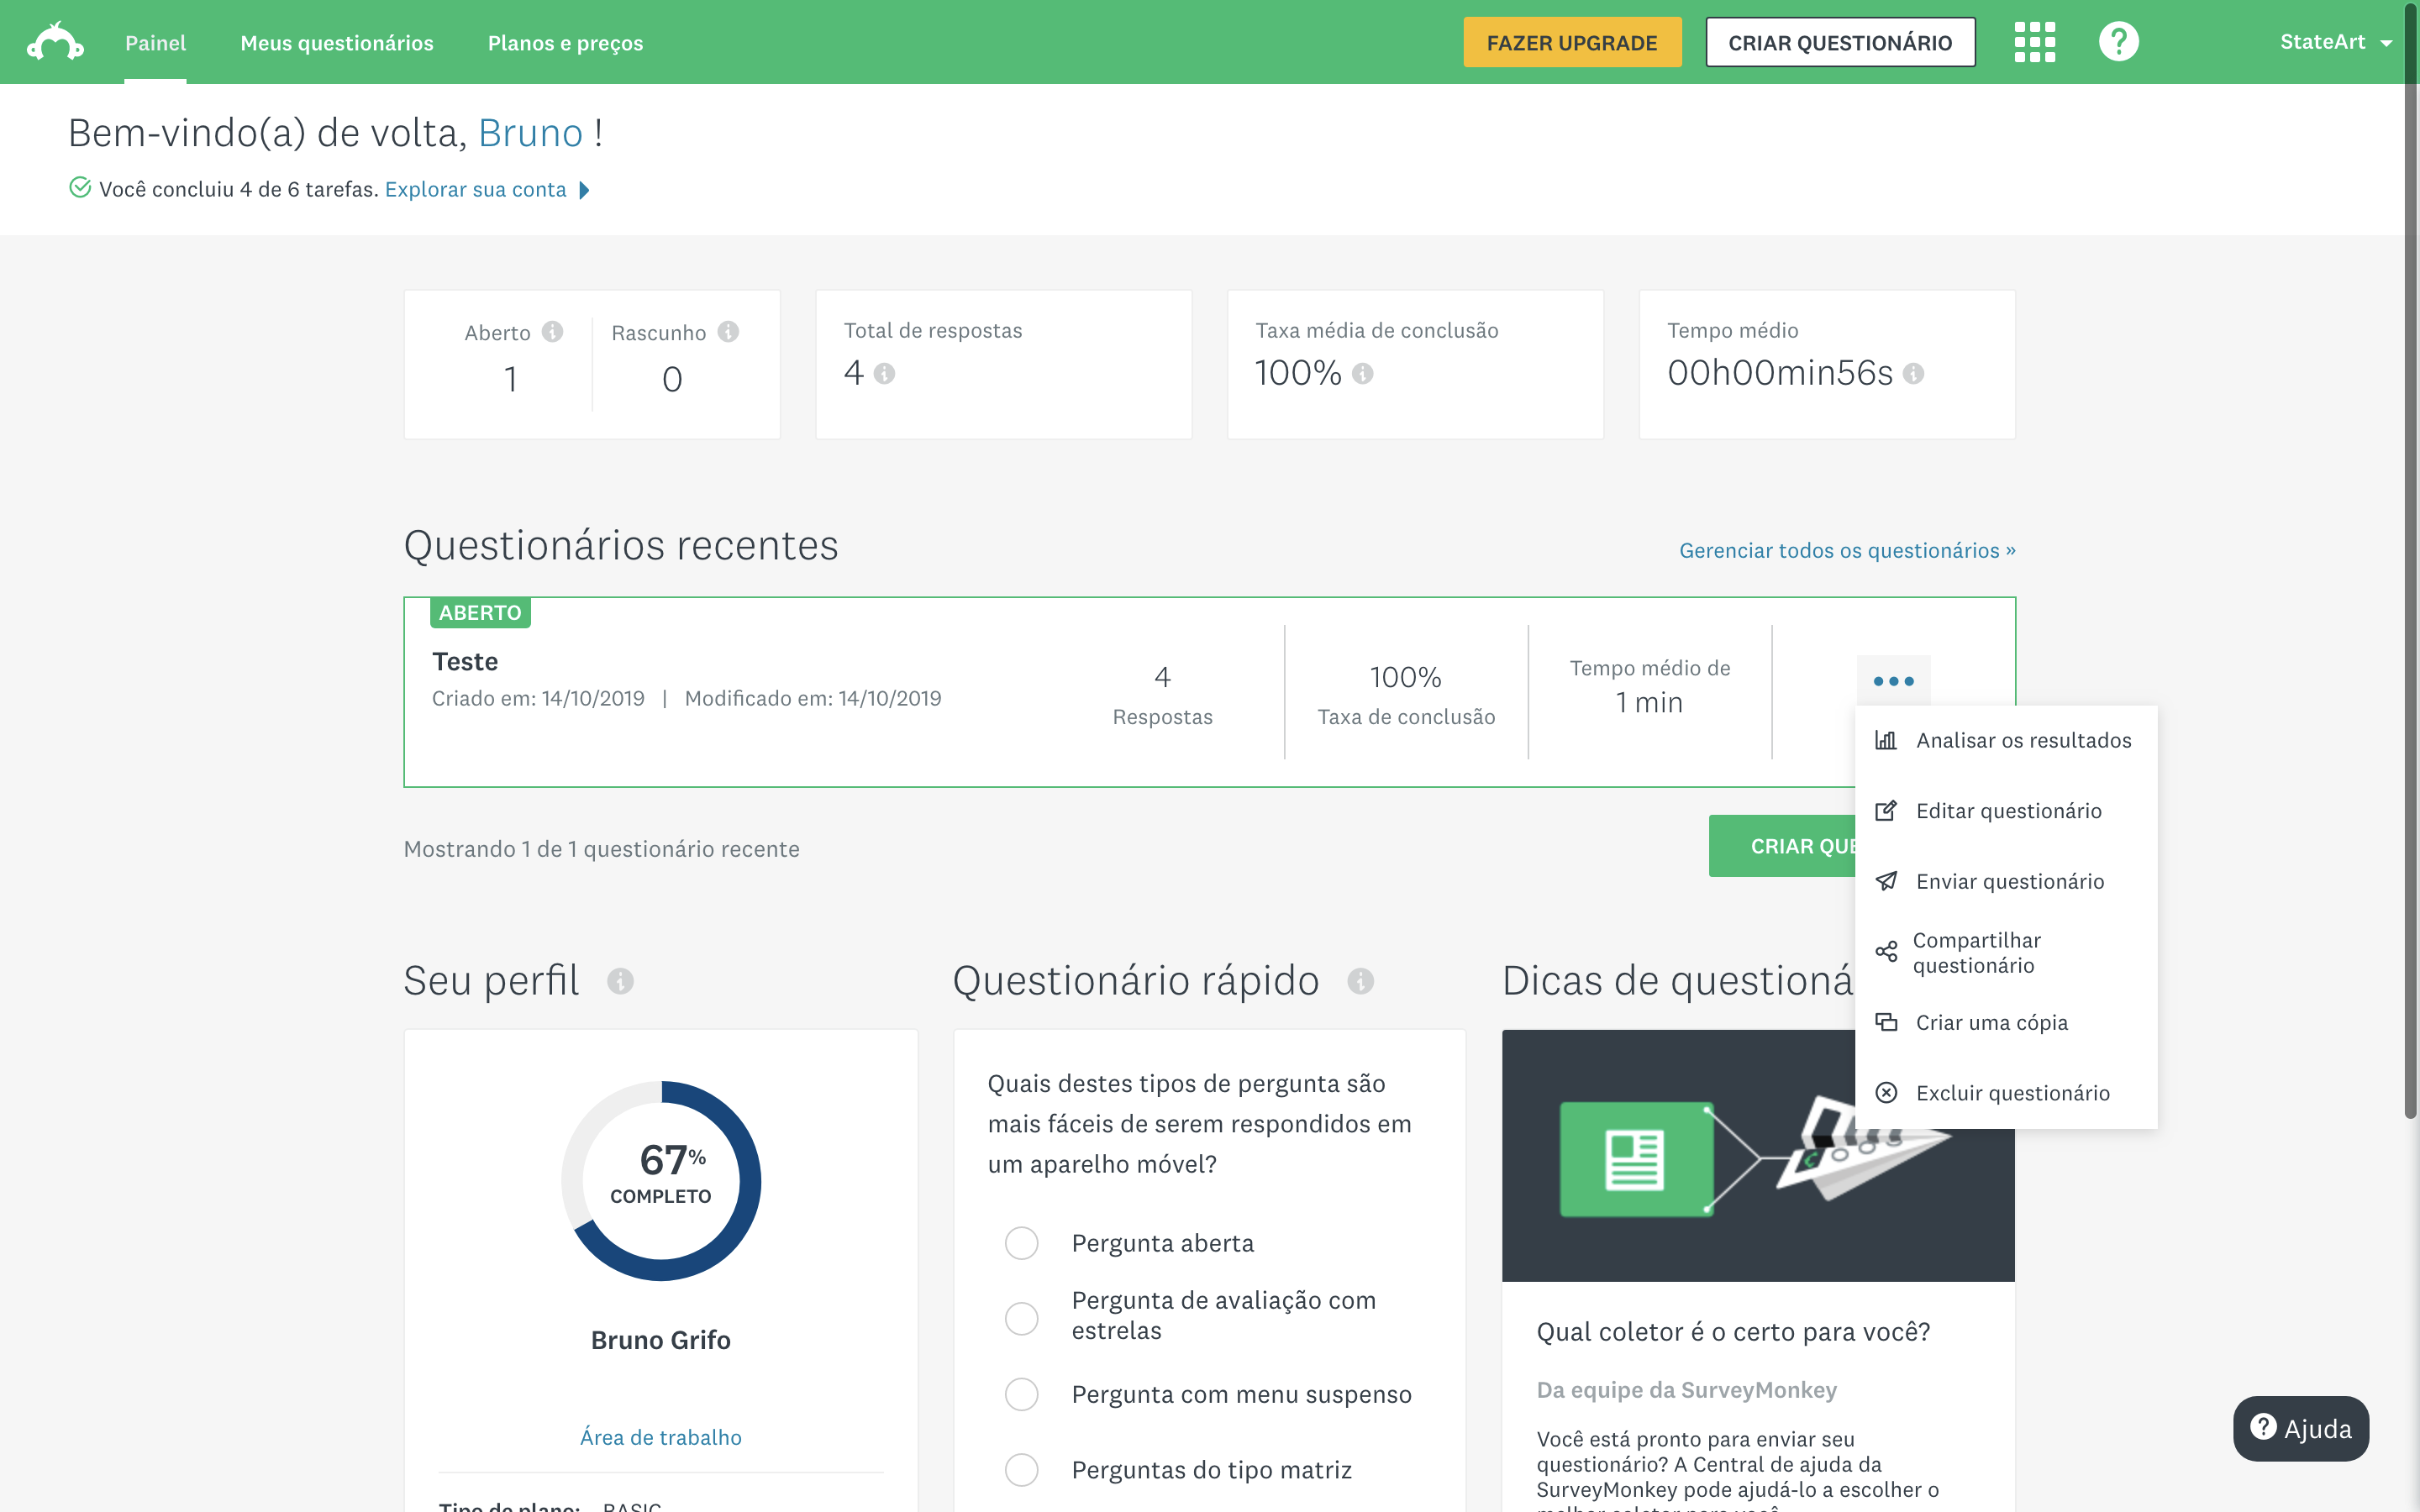
\includegraphics[width=1\textwidth]{img/survey-dashboard}
		\caption{SurveyMonkey - Painel de Controle }
		\label{fig:survey-dashboard}
	\end{center}
\end{figure}

\newpage

\begin{figure}[ht!]
	\begin{center}
		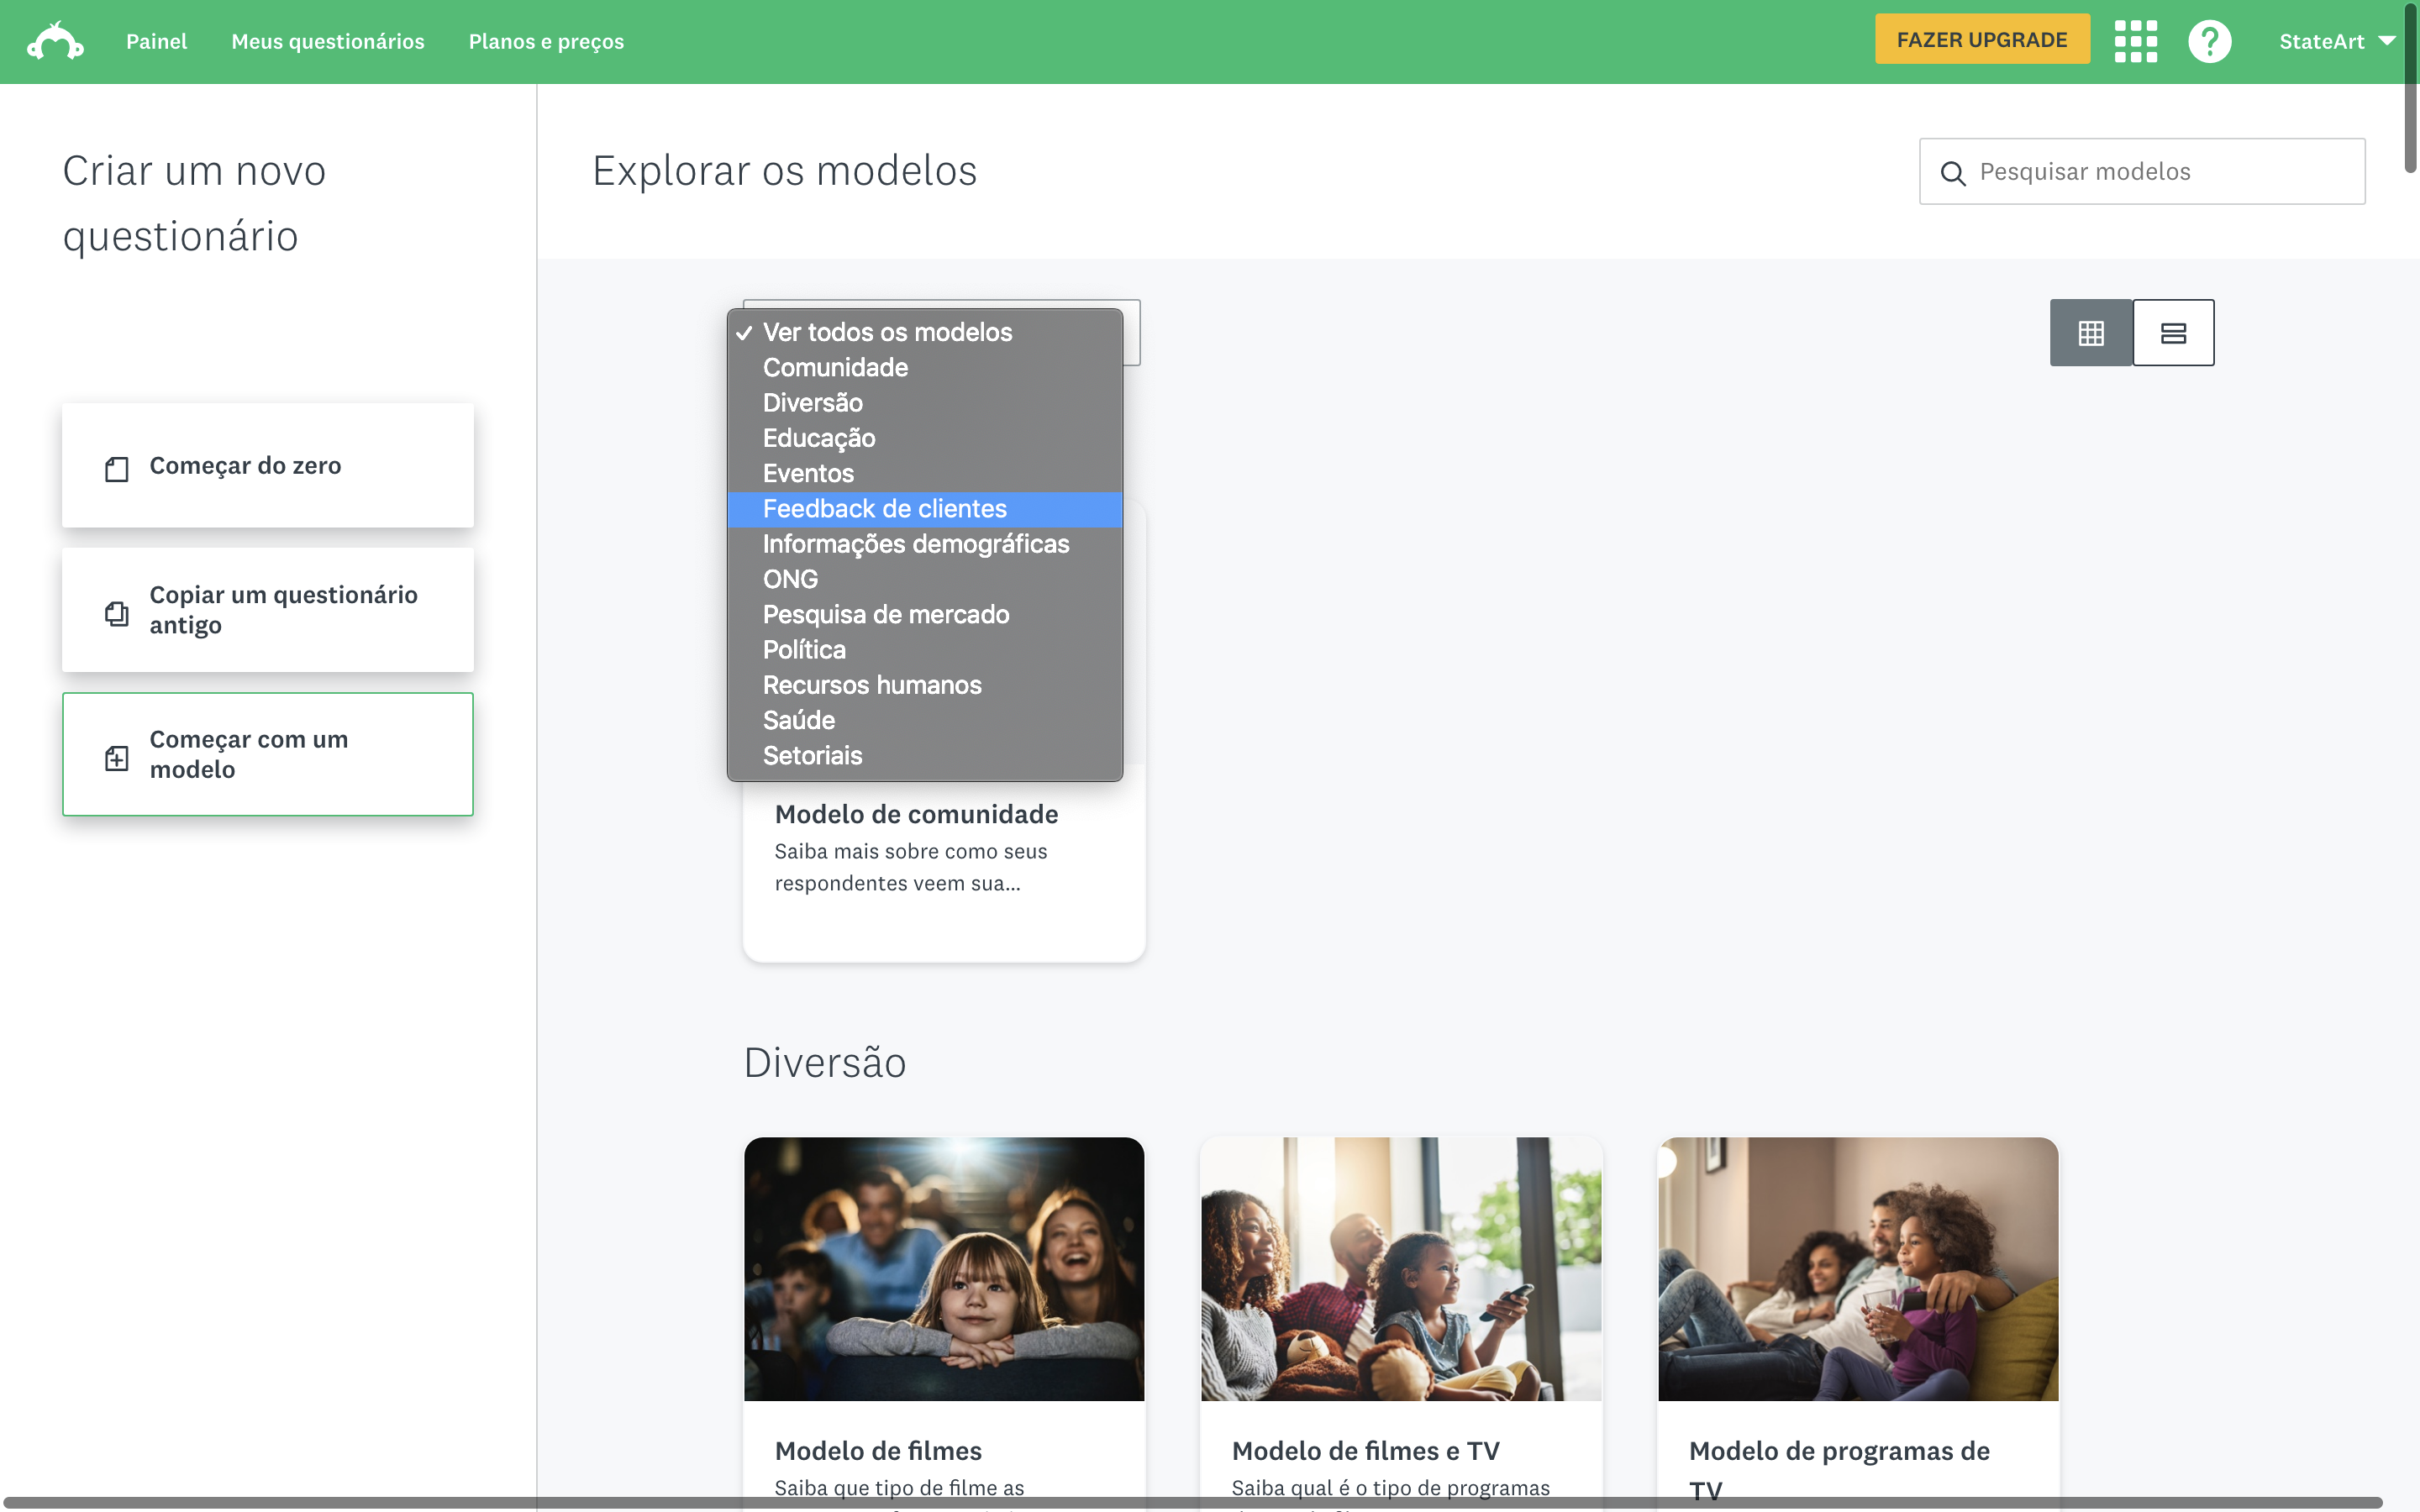
\includegraphics[width=1\textwidth]{img/survey-form-create}
		\caption{SurveyMonkey - Formulários modelo }
		\label{fig:survey-form-create}
	\end{center}
\end{figure}

Quando se inicializa a criação de um novo questionário, a plataforma dá opção de começar do zero ou de utilizar um questionário modelo como podemos ver na Figura \ref{fig:survey-form-create}. Começando um questionário do zero como podemos ver na Figura \ref{fig:survey-form-banck2}, temos acesso a uma série de funcionalidades que vamos explorar e analisar em seguida.

\begin{figure}[ht!]
	\begin{center}
		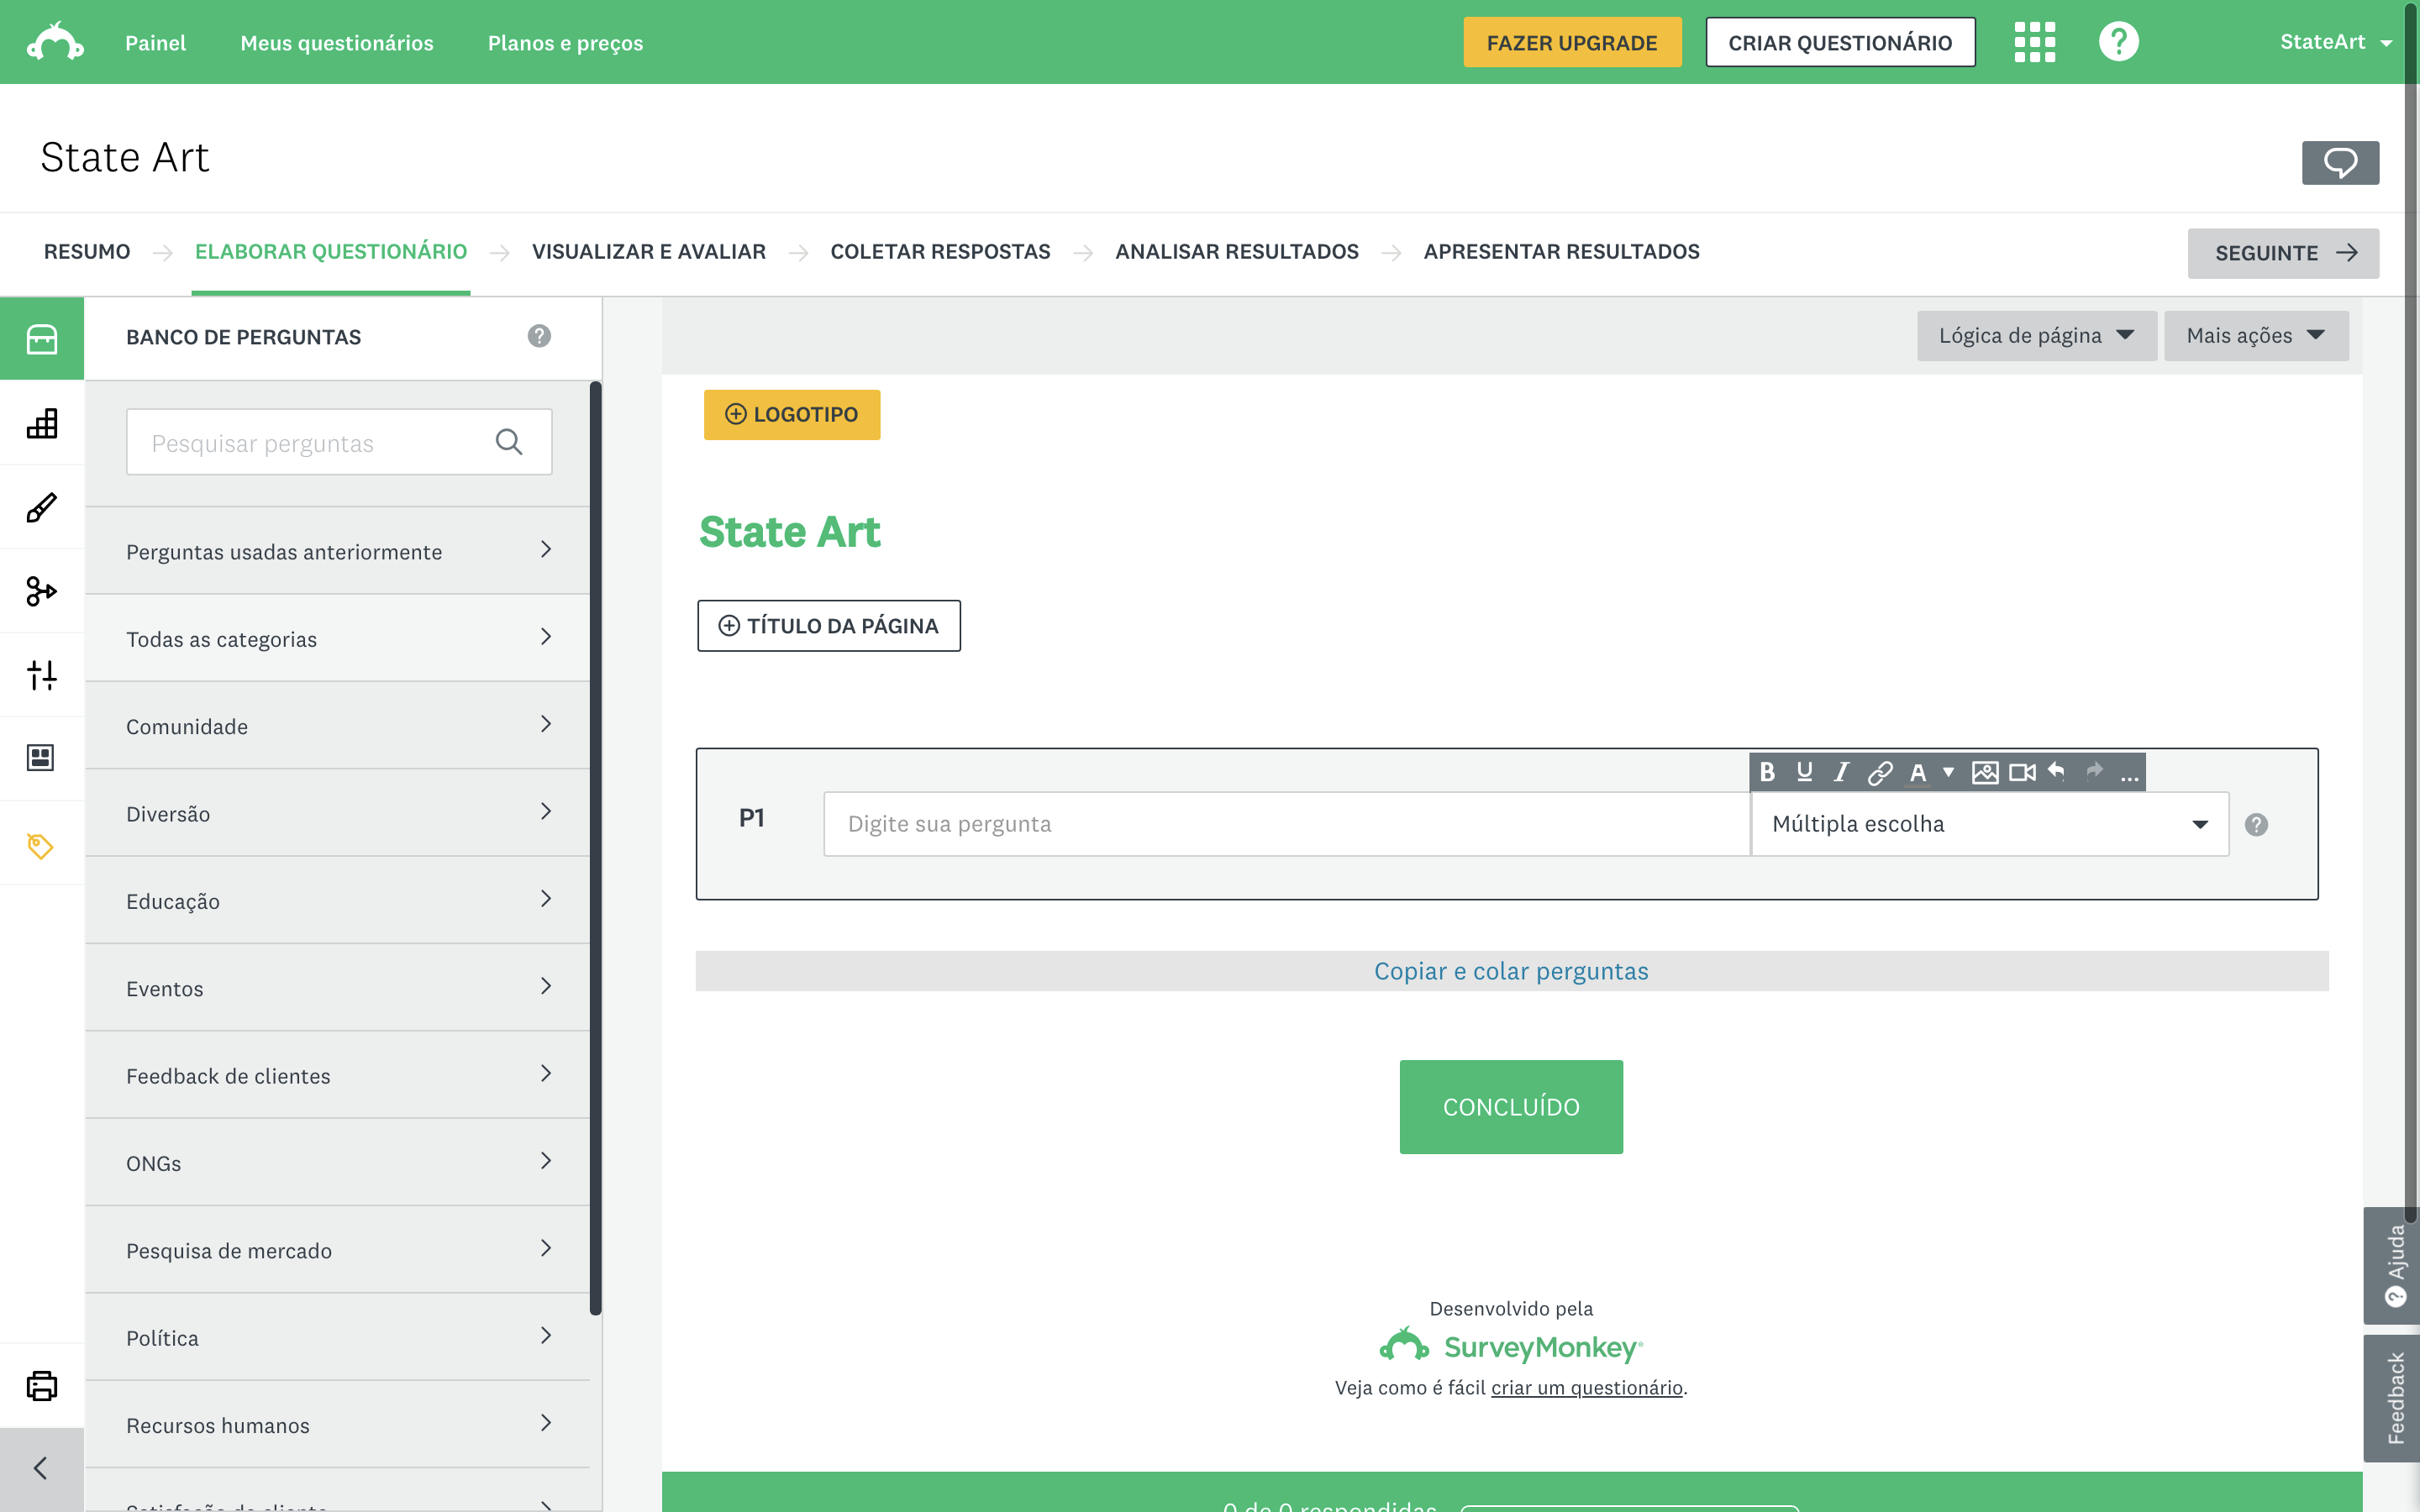
\includegraphics[width=1\textwidth]{img/survey-form-bank2}
		\caption{SurveyMonkey -  Perguntas Modelo}
		\label{fig:survey-form-banck2}
	\end{center}
\end{figure}


\begin{figure}[ht!]
	\begin{center}
		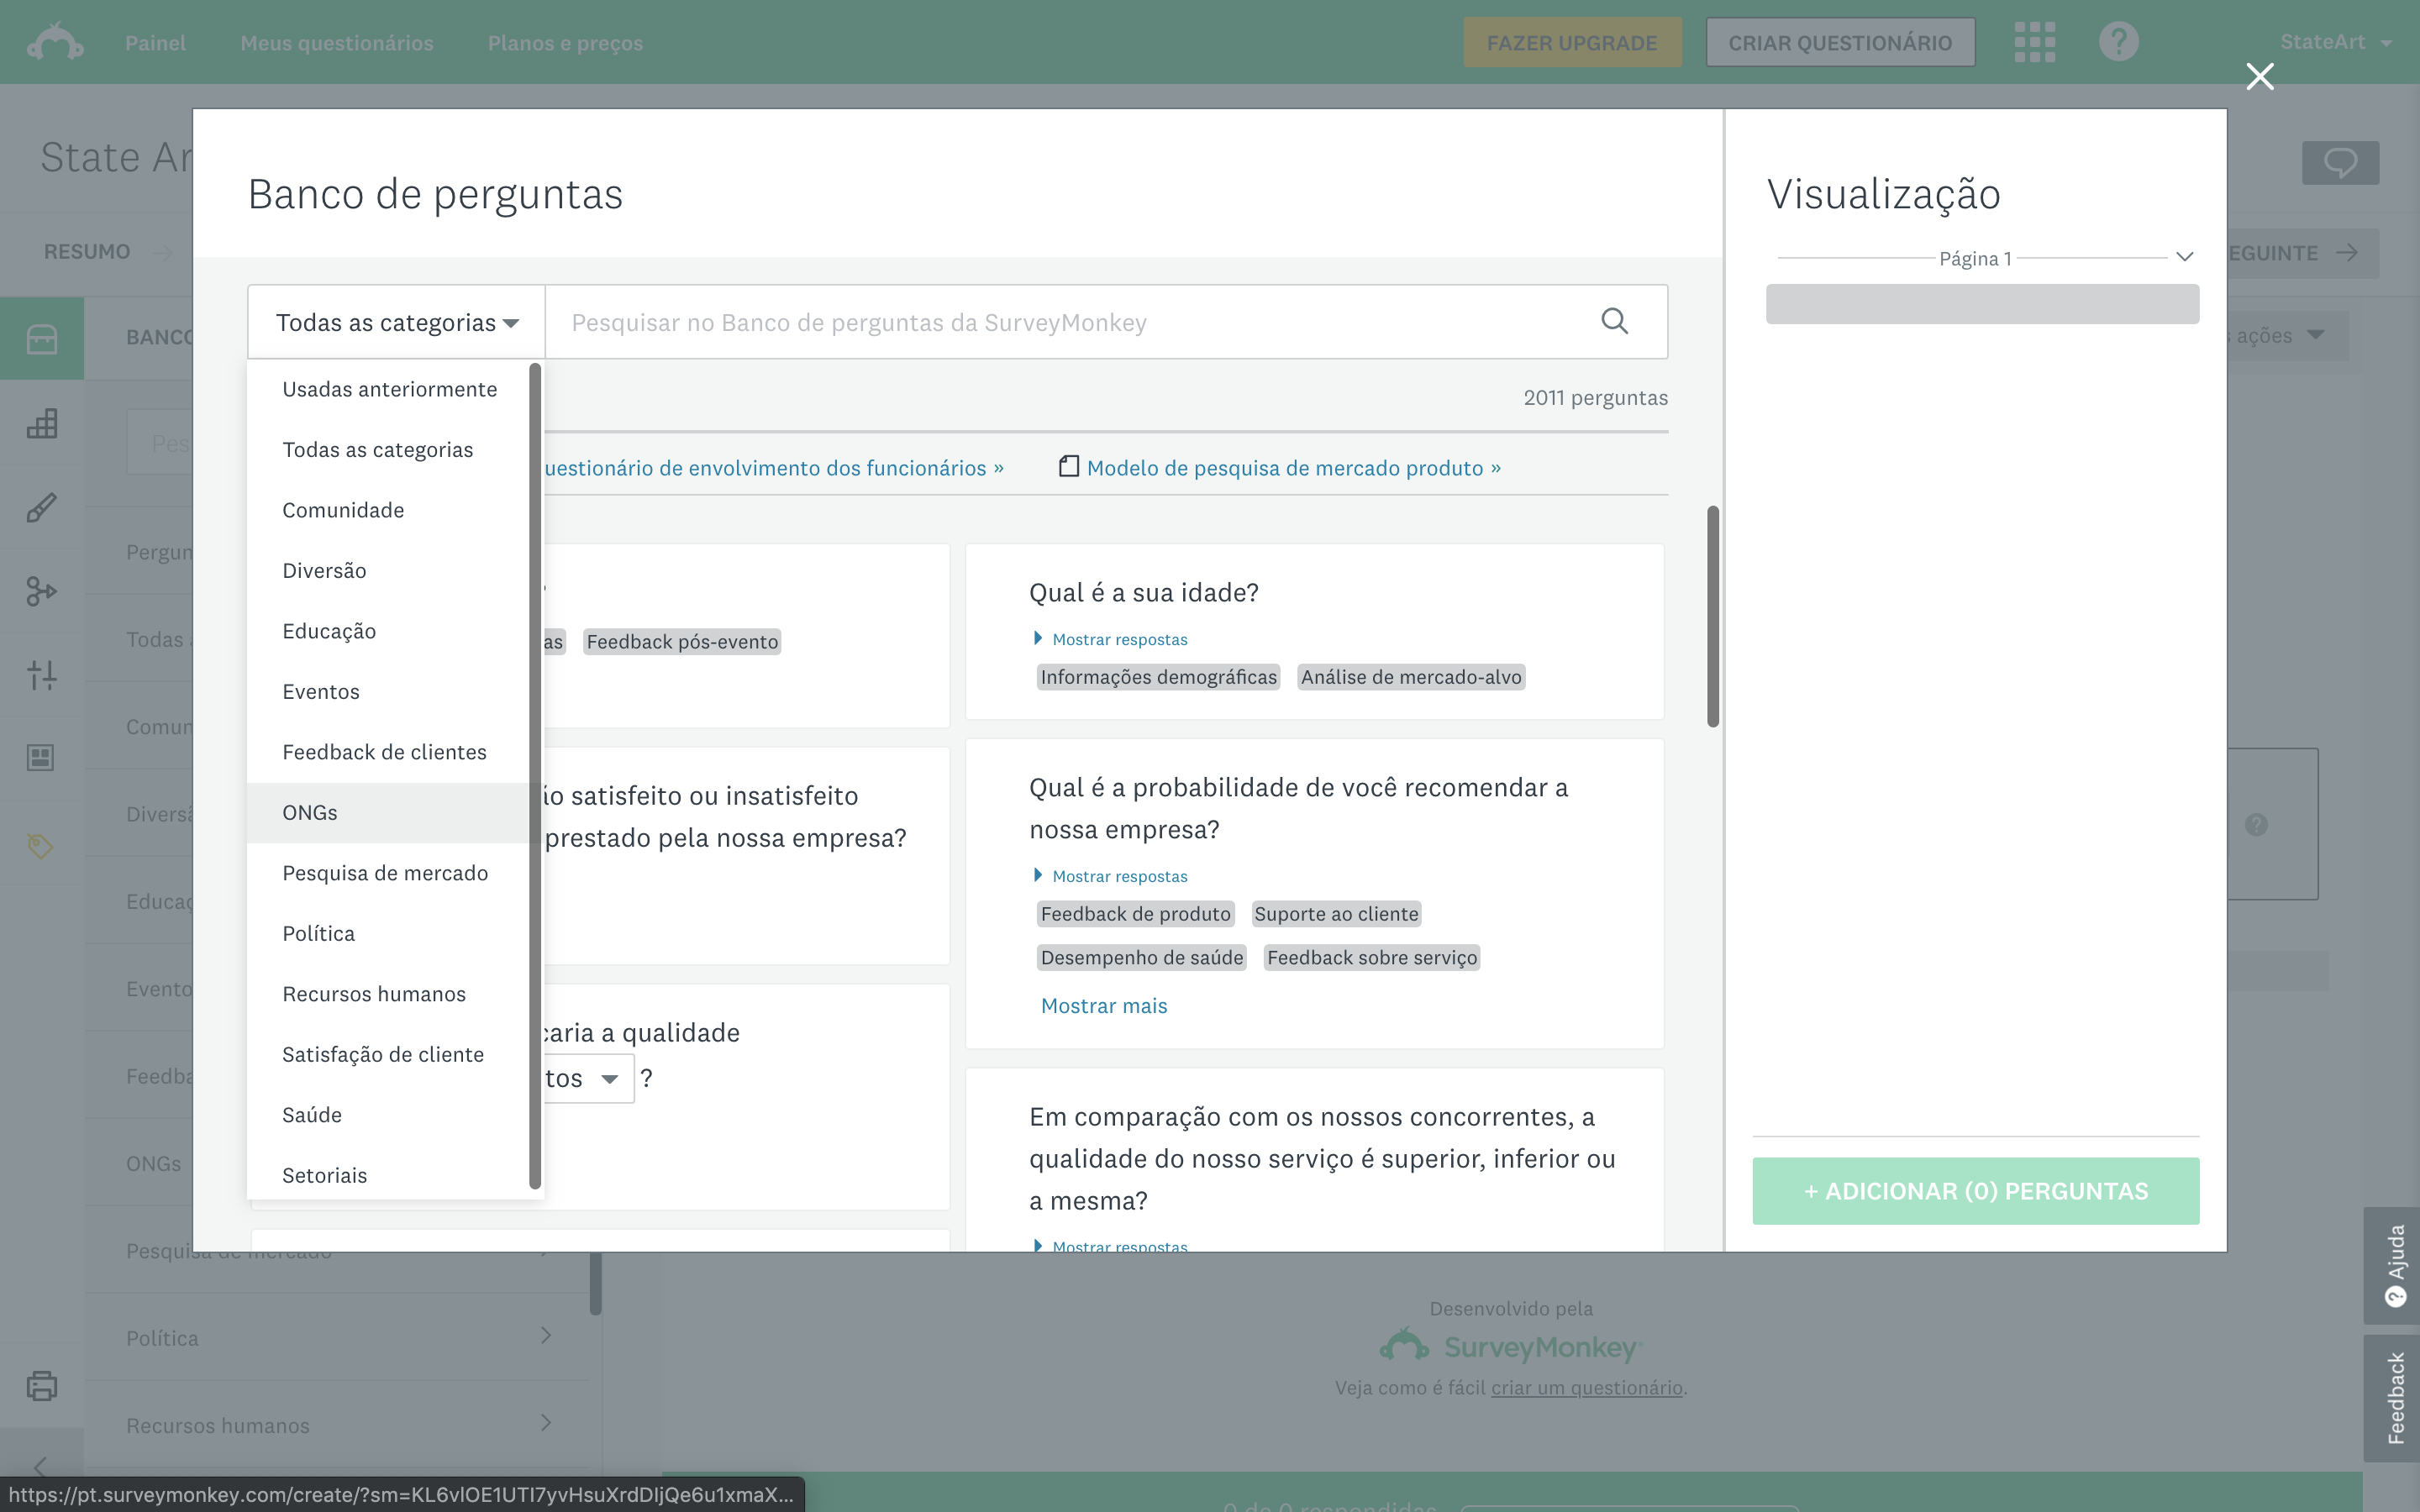
\includegraphics[width=1\textwidth]{img/survey-form-bank1}
		\caption{SurveyMonkey - Perguntas Modelo }
		\label{fig:survey-form-banck1}
	\end{center}
\end{figure}

\newpage

São diversos os elementos que se podem adicionar ou arrastar para o questionário (i. e. perguntas, escolha multipla, imagens...) como representado na Figura \ref{fig:surveymonkey-form-element} e há também um banco de perguntas modelo/recomendações organizadas por categorias como podemos ver na Figura \ref{fig:survey-form-banck2} e \ref{fig:survey-form-banck1}.


\begin{figure}[ht!]
	\begin{center}
		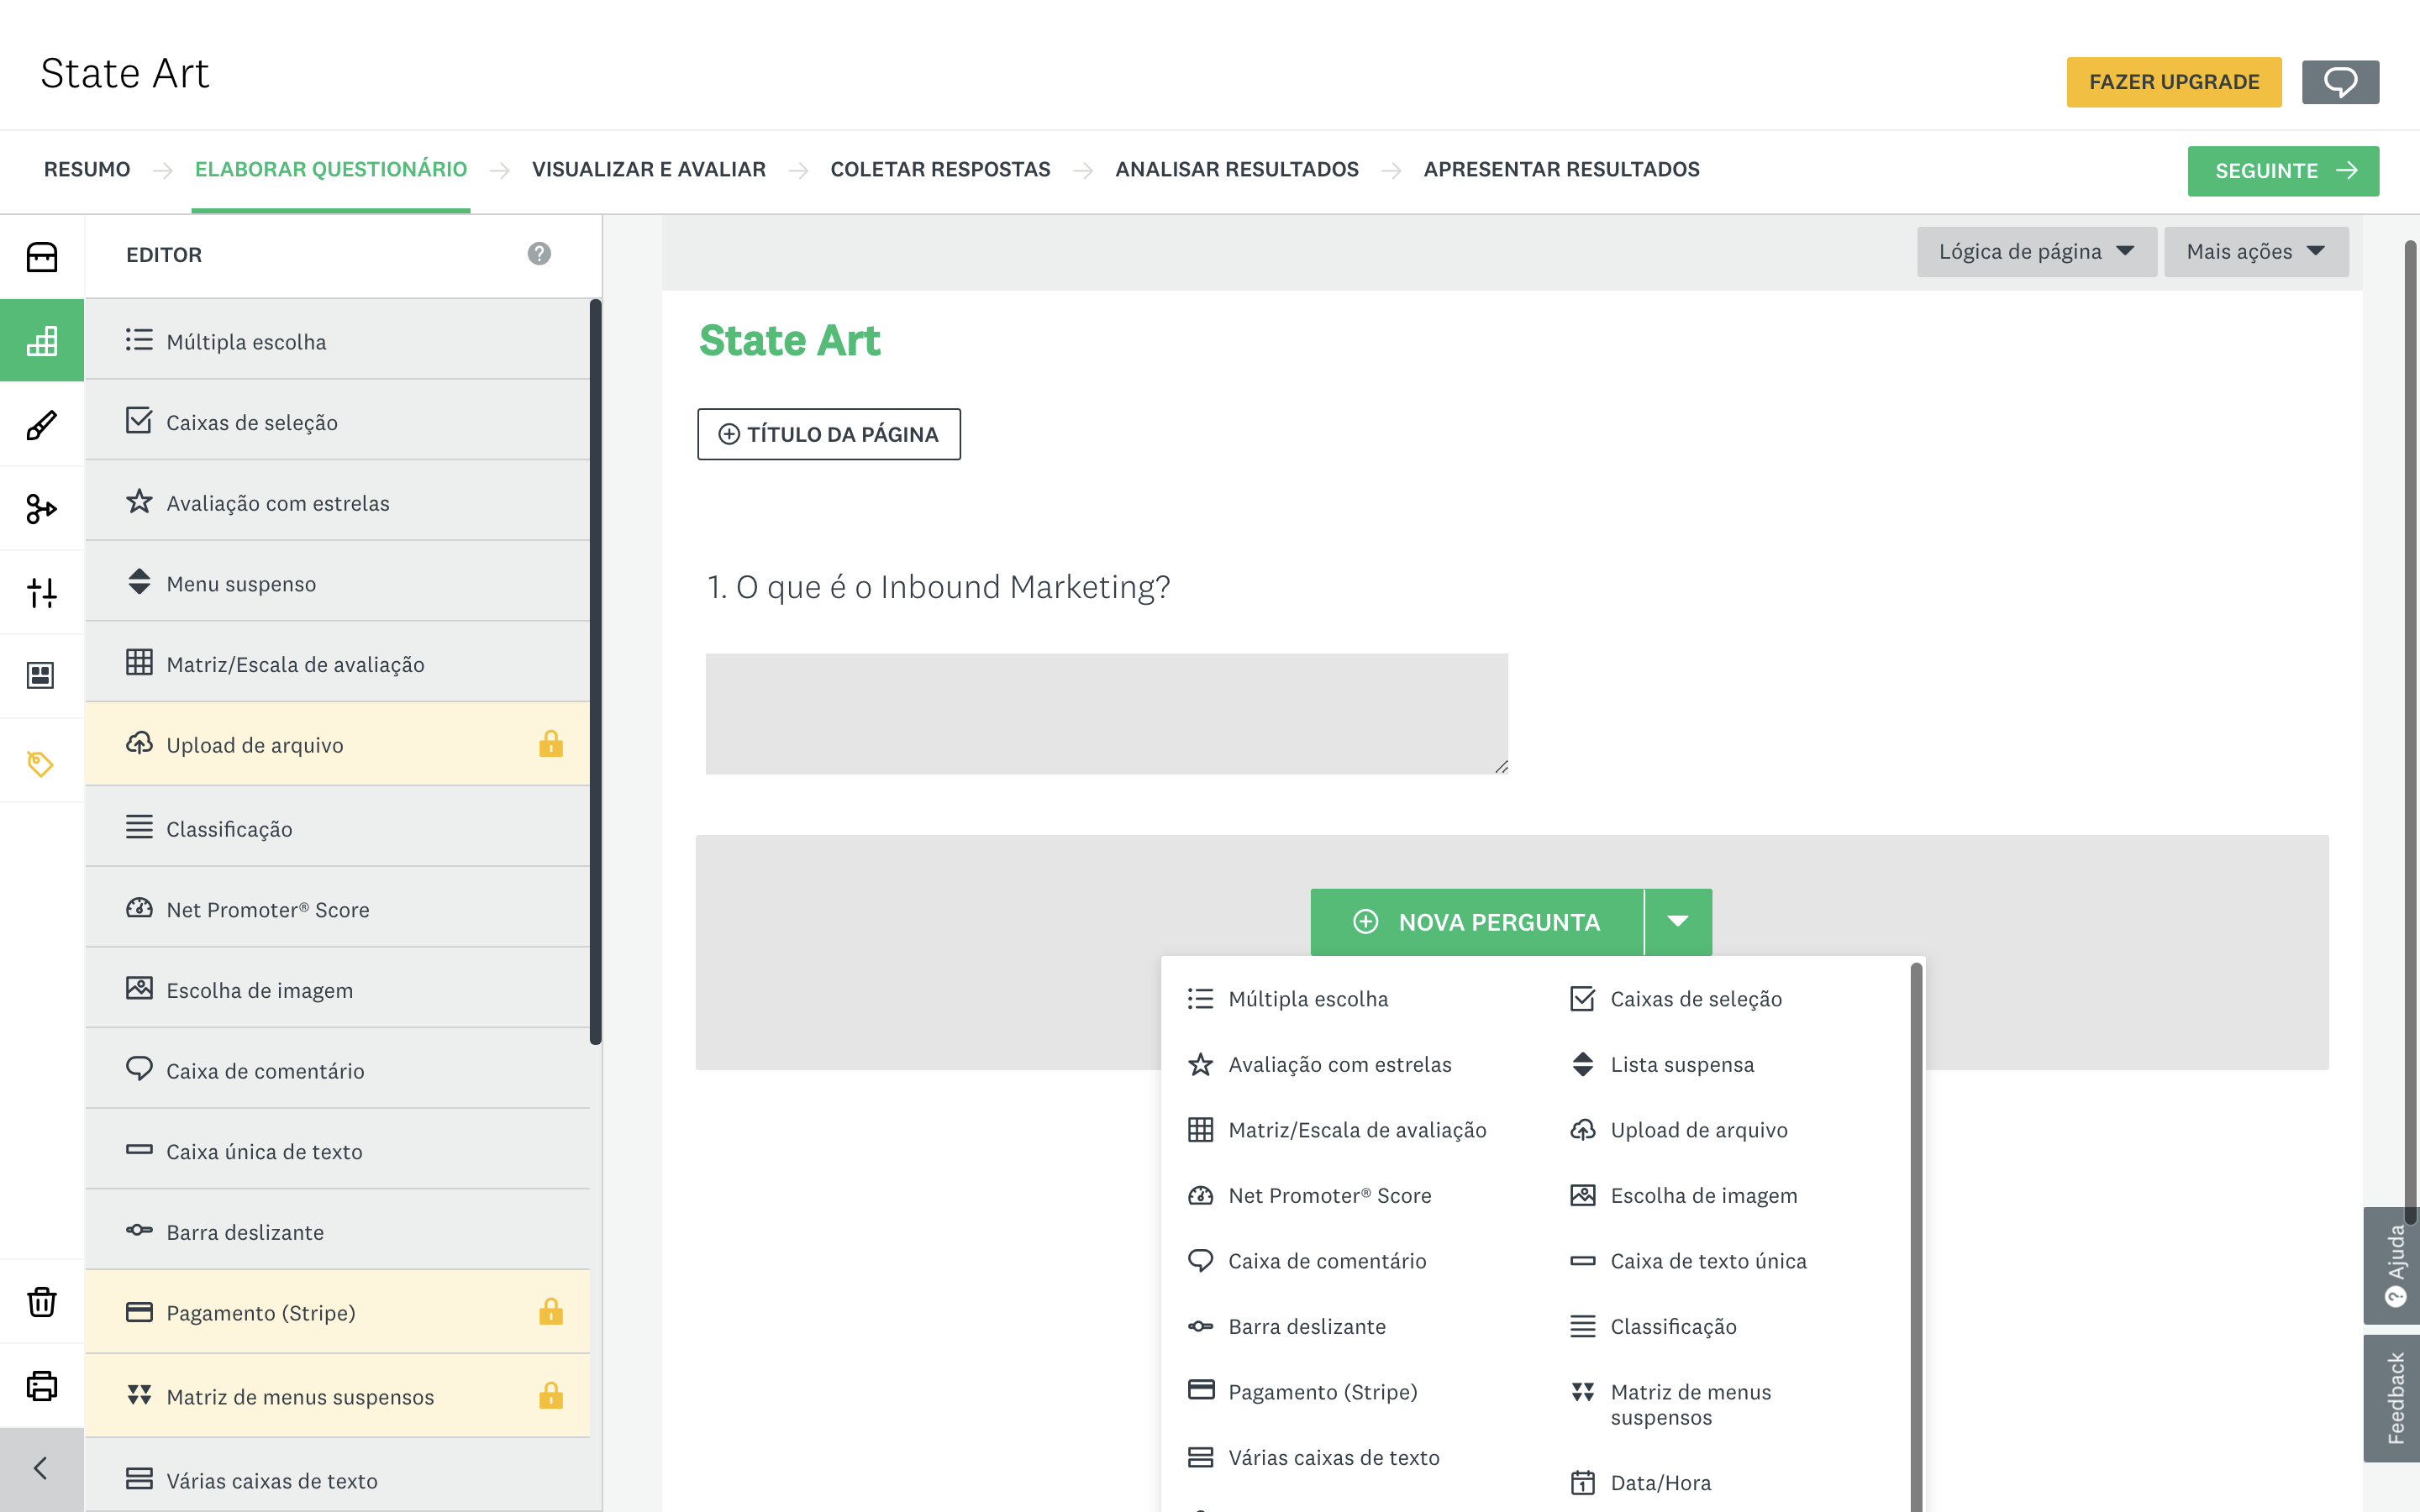
\includegraphics[width=1\textwidth]{img/surveymonkey-form-element}
		\caption{SurveyMonkey - Elementos }
		\label{fig:surveymonkey-form-element}
	\end{center}
\end{figure}

\section{Typeform}
\label{typeform}

\section{Google Form}
\label{googleform}
%-------------------------------------------------------------------------------------------------
\blankpage
%-------------------------------------------------------------------------------------------------

\glsresetall



